\section{Nondeterminism and NP-Completeness}

\subsection{Characterizing NP}

\key{Theorem 6.1.} A set $A$ belongs to NP if and only if there exist a polynomial
$p$ and a binary relation $R$ that is decidable in polynomial time such that for all words
in $\Sigma^*$,
$x \in A \Leftrightarrow \exists y [|y| \le p(|x|) \land R(x, y)]$.

\key{Verifier} Define a verifier for a language $A$ to be an algorithm $V$ such that
$A = \{x |\exists y[V \text{ accepts } \langle x, y \rangle ]\}$.

\key{Corollary 6.1.} NP is the class of all languages A having a polynomial-time
verifier.

\subsection{The Class P}

\subsection{Enumerations}

\key{Definition 6.1.} A class of sets $\mathscr{C}$ is effectively presentable if there is an
effective enumeration $\{M_i\}_i$ of Turing machines such that every Turing machine in the
enumeration halts on all inputs and $\mathscr{C} = \{L(M_i) | i \ge 0\}$.

\key{Theorem 6.2.} There is no effective enumeration of the class of all
deterministic Turing machines that operate in polynomial time. That is,
$S = \{i | \text{DM}_i \text{operates in polynomial time}\}$
is not a computably enumerable set.

\key{Theorem 6.3.} P and NP are effectively presentable:\\
NP = \{L(NP$_i) | i \ge 0\}$;\\
P = \{L(P$_i) | i \ge 0\}$;

\subsection{NP-Completeness}

\key{Definition 6.2.} A set $A$ is many-one reducible in polynomial time to a
set $B$
(notation: $A \le^P_m B$) if there exists a function $f$ that is computable
in polynomial time so that $x \in A \Leftrightarrow f(x) \in B$.

\key{Theorem 6.4.} NP $\ne$ E.

\key{Definition 6.3.} A set $A$ is $\le^P_m$-complete for NP (commonly
called NP-complete) if
\begin{enumerate}
  \item A $\in$ NP;
  \item for every set L $\in$ NP, L $\le^P_m$ A.
\end{enumerate}

\key{Theorem 6.5.} If $A$ is NP-complete, then $A \in P$ if and only if P =
NP.

\key{Universal set for NP} $\mathscr{U} = \{\langle i, x, 0^n \rangle |$ some
computation of NP$_i$ accepts $x$ in fewer than $n$ steps\}

\key{Theorem 6.6.} $\mathscr{U}$ is NP-complete.\\
For each $S\ in$ NP, there is some $i$ such
that $S = L(\text{NP}_i)$. Given $S = L(\text{NP}_i)$, define $f$ so that for
every word $x$, $f(x) = \langle i, x, 0^{p_i(|x|)} \rangle$. Then we have
\begin{align*}
  x \in S &\Leftrightarrow \text{NP}_i \text{accepts } x \\
  &\Leftrightarrow \text{NP}_i \text{accepts } x \text{ in } p_i(|x|) \text{ steps}\\
  &\Leftrightarrow \langle i, x, 0^{p_i(|x|)} \rangle \in \mathscr{U}\\
  &\Leftrightarrow f(x) \in \mathscr{U}
\end{align*}

\subsection{The Cook-Levin Theorem}

\key{Theorem 6.7.} SAT belongs to NP.

\key{Theorem 6.8. (Cook-Levin)} CNF-SAT is an NP-complete problem.

\subsection{More NP-Complete Problems}

\key{Proposition 6.1.} If A is NP-complete, $A \le_m^P B$, and $B \in$ NP, then B is NP-complete.

\key{Corollary 6.2.} SAT is NP-complete.

\subsubsection{The Diagonal Set Is NP-Complete}

\key{$K$} $K = \{i | \text{NP}_i \text{ accepts } i \text{ within } |i| \text{
steps}\}$.

\subsubsection{Some Natural NP-Complete Problems}

\key{Theorem 6.10.} 3SAT is NP-complete.

\key{Vertex cover} A vertex cover of a graph $G = (V, E)$ is a subset $V'$ of
$V$ that, for each edge $(u, v) \in E$, contains at least one of the
adjacent vertices $u$ and $v$.

\key{VERTEX COVER}\\
\textbf{instance} A graph $G = (V, E)$ and a positive integer $k \le ||V||$ .\\
\textbf{question} Is there a vertex cover of size $\le k$ for $G$?

\key{Theorem 6.11.} VERTEX COVER is NP-complete.

\begin{figure}[H]
  \centering
  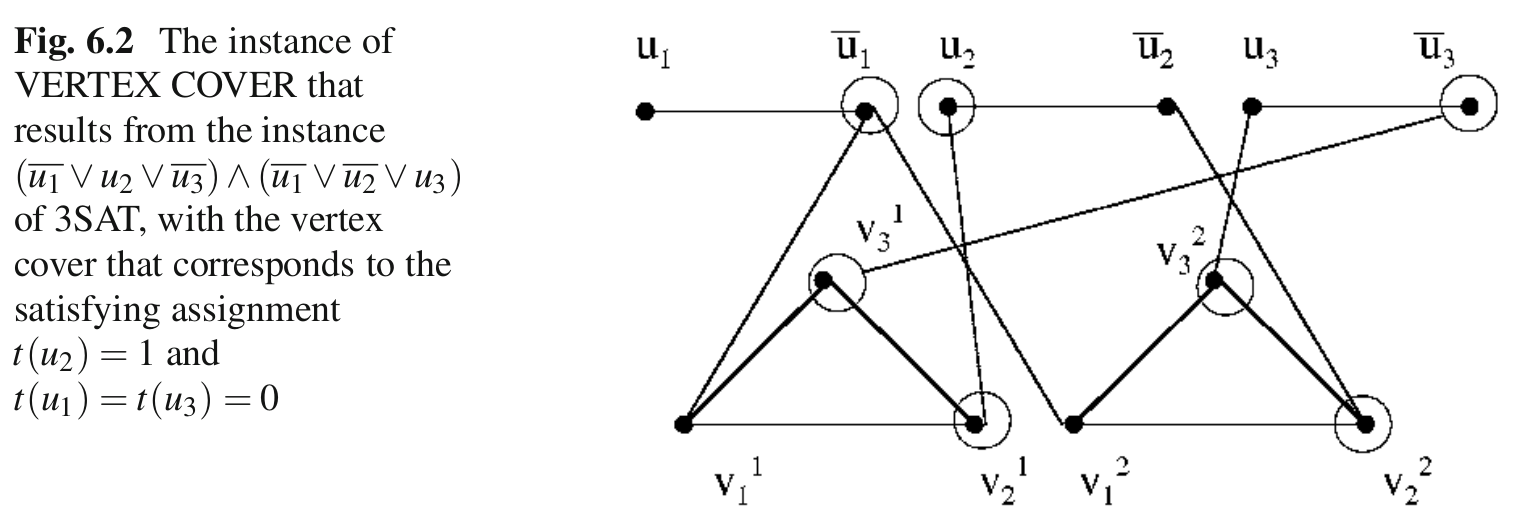
\includegraphics[width=0.96\textwidth]{vertex_cover}
\end{figure}

\key{Clique} A complete subgraph of G

\key{CLIQUE} \\
\textbf{instance} A graph $G = (V, E)$ and a positive integer $j \le ||V||$ .\\
\textbf{question} Does $G$ contain a clique of size $j$ or more?

\key{Theorem 6.12.} CLIQUE is NP-complete.
